\subsection{Unbewachtes Lernen}
\label{subsec:un_lear}
Mit dem konstruierten Datensatz und der zusätzlichen Metrik zur Bestimmung ähnlicher Hotels erfolgt nun die Modellierung. Aufgrund der Unbekanntheit im Vorfeld, welche Hotels miteinander vergleichbar sind, wird ein Modell für unbewachtes Lernen implementiert. Unbewachtes Lernen bezeichnet eine Methode des maschinellen Lernens, bei der der Algorithmus eigenständig und ohne Überwachung Muster sowie Zusammenhänge in den Daten explorativ erkennt \cite{datasolutGmbH.05.02.2024}. Die Grundidee besteht darin, jedes Hotel in einer vergleichbaren Form dem Modell zuzuführen. Dieses Modell erkennt eigenständig Muster und Ähnlichkeiten auf Basis der gegebenen Informationen.
\newline
\newline
Die Evaluation der unterschiedlichen Ansätze und Modelle erfolgt anhand der Benchmark-Hotels, welche in der Sektion zu den Benchmark-Hotels selektiert wurden. Ein Ansatz oder Modell wird als erfolgreich betrachtet, wenn es für die Benchmark-Hotels ein oder mehrere ähnliche Hotels identifiziert, die Korrelationswert von mindestens 0,8 haben.

\subsubsection{Basismodell}
\label{subsubsec:Basismodel}
Ein Basismodell ist im Grundlegenden ein einfaches Modell, das als Referenz in einem ML-Projekt dient. Seine Hauptfunktion besteht darin, die Ergebnisse trainierter Modelle in einen Kontext zu setzen. Basismodelle sind normalerweise wenig komplex und können nur geringe Vorhersagekraft haben. Trotzdem ist ihre Einbeziehung aus verschiedenen Gründen notwendig \cite{Nair.04.04.2022}.
\newline
\newline
Einerseits dient das Basismodell dazu, einen initialen Einstieg in die Modellierung zu ermöglichen, dessen Ergebnisse anschließend mittels der zuvor ausgewählten Metrik evaluiert werden können. Hierbei wird ein vollständiger Workflow in vergleichsweise kurzer Zeit geschaffen. Andererseits fungiert das Basismodell als Referenzpunkt, welcher durch weitere Modelle übertroffen werden soll. Ein beispielhaftes Szenario für ein solches Basismodell könnte ein Empfehlungssystem für Filme sein, bei dem stets die aktuell beliebtesten Filme auf der Plattform angeboten werden.
\newline
\newline
Im vorliegenden Kontext besteht das Basismodell darin, vier zufällige Hotels aus dem Gesamtdatensatz zu extrahieren und diese als ähnlich zu betrachten. Mit dem Basismodell welches vier zufällige Hotels liefert, sieht die Evaluation wie folgt aus:

\begin{figure}[h]
    \centering
    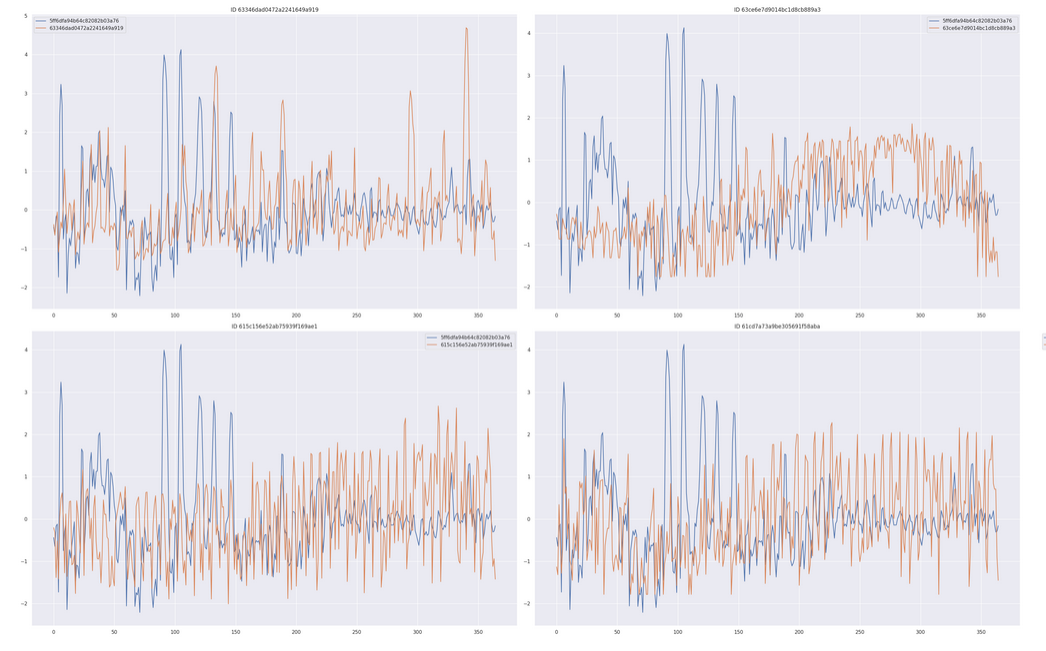
\includegraphics[width=1\textwidth, center]{basismodel_1.png}
    \caption[Basismodell Ergebnisse der RevPAR-Verläufe]{Basismodell Ergebnisse der RevPAR-Verläufe}
    \label{img:basismodell_1}
\end{figure}

\begin{figure}[h]
    \centering
    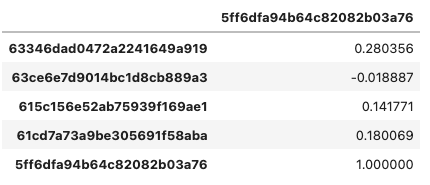
\includegraphics[width=1\textwidth, center]{basismodel_2.png}
    \caption[Basismodell Ergebnisse der RevPAR-Korrelationen]{Basismodell Ergebnisse RevPAR-Korrelationen}
    \label{img:basismodell_2}
\end{figure}

In den Abbildungen \ref{img:basismodell_1} und \ref{img:basismodell_2} sind die Ergebnisse für das Hotel mit der Identifikationsnummer \emph{5ff6dfa94b64c82082b03a76} im Zusammenhang mit dem Basismodell ersichtlich. Sowohl Abbildung \ref{img:basismodell_1} als auch Abbildung \ref{img:basismodell_2} verdeutlichen, dass die vier Hotels, welche vom Basismodell ausgewählt wurden, keine deutliche Ähnlichkeit aufweisen. Des Weiteren zeigt Abbildung \ref{img:basismodell_2} eindeutig, dass das angestrebte Ziel, ein Hotel mit einem Korrelationswert von mindestens 0,8 zu identifizieren, nicht erreicht wurde. Infolgedessen hat das Basismodell die entsprechende Anforderung nicht erfüllt.


\subsubsection{DBScan Modell}
\label{subsubsec:dbscan}
Die erste Idee nach dem Basismodell, um ähnliche Hotels zu finden, ist es den weitverbreiteten \emph{Density-Based Spatial Clustering of Applications with Noise-Algorithmus} zu nutzen. Der \emph{Density-Based Spatial Clustering of Applications with Noise-Algorithmus} kurz DBScan ist ein leistungsfähiger Ansatz zur Clusteranalyse, der darauf abzielt, Cluster in Datensätzen mit variabler Dichte zu identifizieren. Anders als klassische Clustering-Algorithmen, die auf geometrischen Formen oder Distanzmetriken basieren, nutzt DBScan die Dichte der Datenpunkte, um Cluster zu identifizieren \cite{6814687}.
\newline
\newline
Die Identifikation von Clustern innerhalb eines Datensatzes erfordert vom DBScan-Algorithmus zwei wesentliche Informationen:

\begin{itemize}
    \item Mindestanzahl an Datenpunkten für die Bildung eines Clusters.
    \item Maximale Entfernung, in der Datenpunkte voneinander liegen dürfen.
\end{itemize}

Ein Vorteil des DBScan-Algorithmus besteht darin, dass keine vorherige Festlegung darüber getroffen werden muss, wie viele Cluster am Ende resultieren sollen. Es genügt die Angabe dieser beiden genannten Informationen, um die Bildung von Clustern zu ermöglichen.
\newline
\newline
Die zugrunde liegende Hypothese dieser Methodik besagt, dass der DBScan-Algorithmus alle ähnlichen Hotels in einem Cluster zusammenführt.

\paragraph{Vorbereitung des Datensatzes} 
Der in Abbildung \ref{img:all_features_4} dargestellte Datensatz enthält sowohl numerische als auch kategoriale Daten. Da der DBScan-Algorithmus ausschließlich mit numerischen Daten arbeiten kann, ist es erforderlich, den vorhandenen Datensatz vor der Anwendung des Algorithmus zu transformieren. Zu diesem Zweck wird eine Pipeline erstellt, die auf den gesamten Datensatz angewendet wird. In einem ersten Schritt werden die kategorialen Daten mithilfe von \emph{One-Hot-Encoding} umgewandelt. Darüber hinaus erfolgt eine Skalierung der bereits vorhandenen numerischen Daten.
\newline
\newline
Die Struktur der Pipeline ist wie folgt:

\begin{lstlisting}[language=Python, label=lst:pipeline, caption=Datensatz Pipeline]
from sklearn.compose import ColumnTransformer
from sklearn.pipeline import make_pipeline
from sklearn.preprocessing import StandardScaler, OneHotEncoder

numerical_features = ['median_min', 'median_max']
categorical_features = ['art', 'region2']
    
numerical_pipeline = make_pipeline(StandardScaler())
    
categorical_pipeline = make_pipeline(OneHotEncoder())
    
preprocessor = ColumnTransformer(
    transformers=[
        ('num', numerical_pipeline, numerical_features),
        ('cat', categorical_pipeline, categorical_features)
    ])
    
    
pipeline = make_pipeline(preprocessor)
\end{lstlisting}

Die in dem Listing \ref{lst:pipeline} gezeigte Pipeline kann nun auf Datensatz angewendet werden. Dazu muss die Pipeline zunächst du den Datensatz abgestimmt werden, um dann den Datensatz zu Transformieren. Dies wird mit dem folgenden Listing veranschaulicht:

\begin{lstlisting}[language=Python, label=lst:pipeline2, caption=Ausführung der Pipeline auf dem Datensatz]
# Anpassen der Daten an die Pipeline
pipeline.fit(df)

# Transformieren der Daten
transformed_df = preprocessor.transform(df)

# Erstelle einen DataFrame aus den transformierten Daten
model_df = pd.DataFrame(transformed_df.toarray(), 
                        columns=numerical_features + 
                            list(preprocessor.named_transformers_['cat']
                                                .named_steps['onehotencoder']
                                                .get_feature_names_out(categorical_features)))
\end{lstlisting}

\paragraph{Modellbildung} 
Nach erfolgter Transformation des Datensatzes kann dieser in den DBScan-Algorithmus eingegeben werden, um die Cluster zu generieren. Als Mindestanzahl an Datenpunkten für ein Cluster wird der Wert 2 festgelegt, da stets Paare von zwei Hotels gefunden werden sollen. Das Auffinden der Cluster erfolgt daraufhin lediglich durch einen Aufruf.

\begin{lstlisting}[language=Python, label=lst:dbscan, caption=Ausführung des DBScan-Algorithmus]
from sklearn.cluster import DBSCAN

# Define variables
eps = 0.8
min_samples = 2 

# Create the DBScan algorithm
dbscan = DBSCAN(eps=eps, min_samples=min_samples)

# Add Cluster to df
model_df['Cluster'] = dbscan.fit_predict(model_df)
\end{lstlisting}

Das Listing \ref{lst:dbscan} veranschaulicht die Initialisierung des DBScan-Algorithmus sowie die Erzeugung der individuellen Cluster. Diese Cluster werden anschließend der Datenreihe in der Spalte \emph{Cluster} zugeordnet.
\newline
\newline
In einem nachfolgenden Schritt können die erstellten Cluster wie folgt visualisiert werden:

\begin{figure}[h]
    \centering
    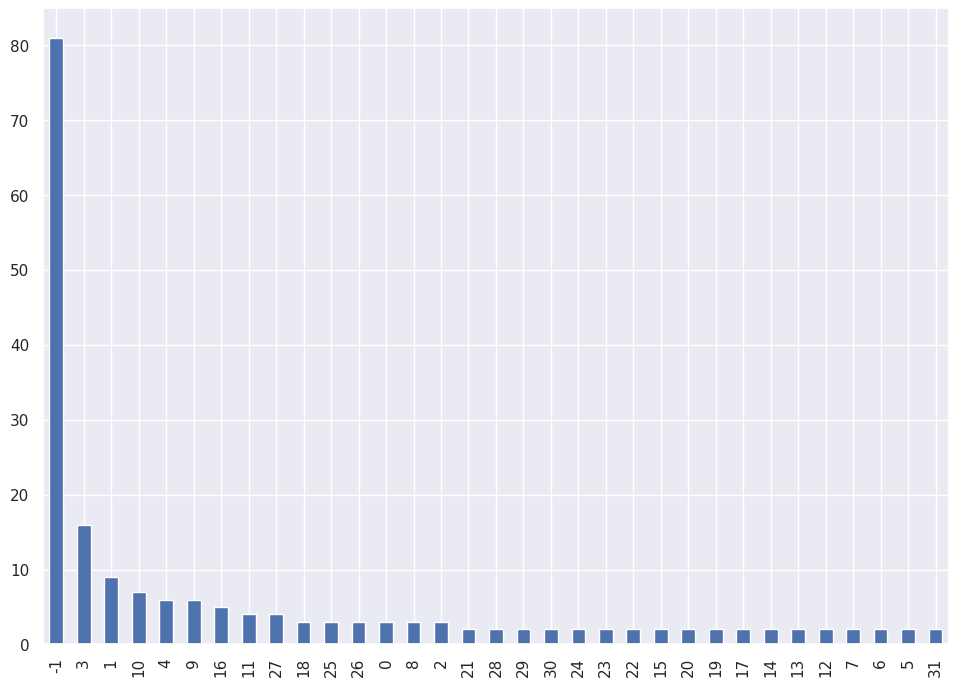
\includegraphics[width=0.85\textwidth, center]{cluster.png}
    \caption[DBScan Clusters]{DBScan Clusters}
    \label{img:cluster}
\end{figure}

Abbildung \ref{img:cluster} zeigt die verschiedenen Cluster, die durch den DBScan-Algorithmus erstellt wurden. Es sind insgesamt 32 Cluster zu erkennen, beginnend mit Cluster 0, sowie eine weitere Kategorie \emph{-1}, die anzeigt, dass für diese Hotels kein Cluster gefunden wurde. Bemerkenswert ist dabei, dass die Mehrheit dieser Hotels keinem Cluster zugeordnet wurde.
\newline
\newline
Ungeachtet dieser Beobachtung soll im nächsten Schritt überprüft werden, welche Hotels mit dem Benchmark-Hotel in einem Cluster vorhanden sind. Hierfür müssen die Hotel-IDs in einer zusätzlichen Spalte dem Dataframe hinzugefügt werden. Die nachfolgende Code-Sequenz im angegebenen Listing ermöglicht die Identifikation der Hotels, die mit dem Benchmark-Hotel in einem Cluster sind.

\begin{lstlisting}[language=Python, label=lst:dbscan_values, caption=Finden alle Hotel ID´s innerhalb des gleichen Clusters]
# Add hotel ids to the dataset with the clusters
model_df['hotel_id'] = df.index

# Get the row for the benchmark hotel
benchmark_row = model_df[model_df["hotel_id"] == str(benchmark_hotel_id)]

# Get the Cluster value of the benchmark hotel
benchmark_cluster = list(benchmark_row["Cluster"].values)[0]

# Get the rows with the same cluster as the benchmark hotel
benchmark_cluster_df = model_df[model_df["Cluster"] == benchmark_cluster]

# Get the hotel ids 
hotel_ids = list(benchmark_cluster_df["hotel_id"].values)
\end{lstlisting}

Die Variable \emph{hotel\_ids} enthält nun sämtliche Hotel-IDs, die zusammen mit dem Benchmark-Hotel in einem Cluster verortet sind. Initial besteht das Interesse darin, die identifizierten Hotels zu visualisieren. Daher soll im Anschluss angezeigt werden, welche Merkmale die identifizierten Hotels aufweisen.

\begin{figure}[h]
    \centering
    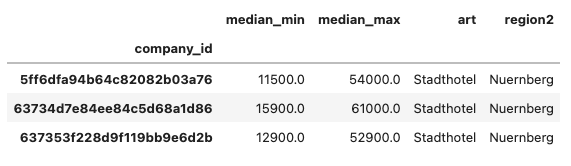
\includegraphics[width=1\textwidth, center]{dbscan_hotels_1.png}
    \caption[Gefundene Hotels für das erste Benchmark-Hotel mit dem DBScan-Algorithmus]{Gefundene Hotels für das erste Benchmark-Hotel mit dem DBScan-Algorithmus}
    \label{img:dbscan_hotels_1}
\end{figure}

Die Hotels, die im identifizierten Cluster zu finden sind, weisen tatsächlich Ähnlichkeiten zu den Merkmalen auf, die das Benchmark-Hotel mit der ID \emph{5ff6dfa94b64c82082b03a76} charakterisieren. Da die Aussagekraft eines einzelnen Hotels begrenzt ist, soll das zweite Benchmark-Hotel ebenfalls mit einbezogen werden. Hierbei sollen auch für dieses Hotel zunächst die identifizierten Hotels anhand ihrer Merkmale bewertet werden.

\begin{figure}[h]
    \centering
    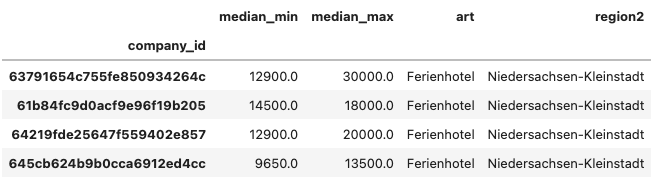
\includegraphics[width=1\textwidth, center]{dbscan_hotels_2.png}
    \caption[Gefundene Hotels für das zweite Benchmark-Hotel mit dem DBScan-Algorithmus]{Gefundene Hotels für das zweite Benchmark-Hotel mit dem DBScan-Algorithmus}
    \label{img:dbscan_hotels_2}
\end{figure}

Unter Berücksichtigung des zweiten Hotels wird ersichtlich, dass der DBScan Hotels mit ähnlichen Merkmalen identifiziert. Dennoch lässt sich anhand der vorliegenden Merkmale nicht eindeutig feststellen, ob diese Hotels tatsächlich ähnliche Verläufe in Bezug auf den RevPAR aufweisen.

\paragraph{Evaluation}
Angesichts der Tatsache, dass allein anhand der Merkmale keine klare Aussage über die tatsächliche Ähnlichkeit der Hotels getroffen werden kann, erfolgt in der nachfolgenden Sektion eine Evaluierung der beiden Benchmark-Hotels. 
\newline
\newline
Der Beginn dieser Evaluierung erfolgt mit dem Hotel, das die ID \emph{5ff6dfa94b64c82082b03a76} trägt. Die Ergebnisse dieser Evaluation werden im Folgenden dargestellt:

\begin{figure}[h]
    \centering
    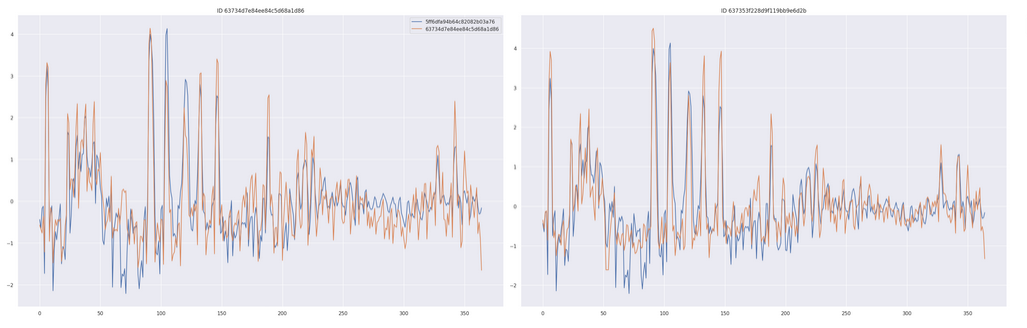
\includegraphics[width=1\textwidth, center]{dbscan_results_1.png}
    \caption[DBScan Ergebnisse der RevPAR-Verläufe für das erste Benchmark-Hotel]{DBScan Ergebnisse der RevPAR-Verläufe für das erste Benchmark-Hotel}
    \label{img:dbscan_results_1}
\end{figure}

\begin{figure}[h]
    \centering
    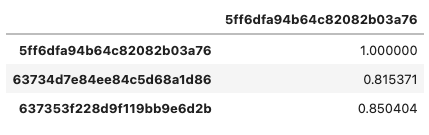
\includegraphics[width=1\textwidth, center]{dbscan_results_1_1.png}
    \caption[DBScan Ergebnisse der RevPAR-Korrelationen für das erste Benchmark-Hotel]{DBScan Ergebnisse der RevPAR-Korrelationen für das erste Benchmark-Hotel}
    \label{img:dbscan_results_1_1}
\end{figure}

Die Abbildungen \ref{img:dbscan_results_1} und \ref{img:dbscan_results_1} verdeutlichen, dass die identifizierten Hotels die Voraussetzungen für einen Korrelationswert von mindestens 0,8 erfüllen. Die Ergebnisse für das Hotel mit der ID \emph{5ff6dfa94b64c82082b03a76} erweisen sich demnach als zufriedenstellend. Allerdings ist eine gewisse Skepsis angebracht, da es auch rein zufällig sein könnte, dass diese Hotels Ähnlichkeiten in Bezug auf den RevPAR Verlauf aufweisen. Aus diesem Grund soll die gleiche Evaluation auch mit dem zweiten Hotel, welches die ID \emph{645cb624b9b0cca6912ed4cc} trägt, durchgeführt werden.

\begin{figure}[h]
    \centering
    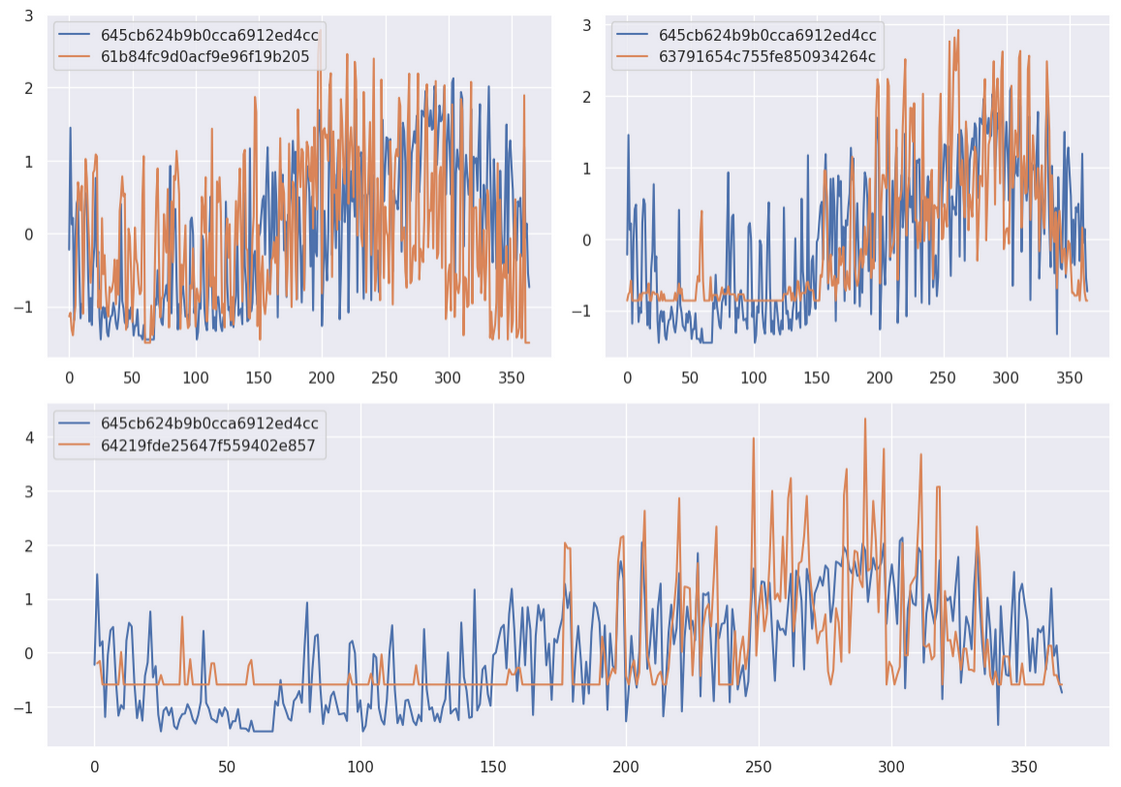
\includegraphics[width=1\textwidth, center]{dbscan_results_2.png}
    \caption[DBScan Ergebnisse der RevPAR-Verläufe für das zweite Benchmark-Hotel]{DBScan Ergebnisse der RevPAR-Verläufe für das zweite Benchmark-Hotel}
    \label{img:dbscan_results_2}
\end{figure}

\begin{figure}[h]
    \centering
    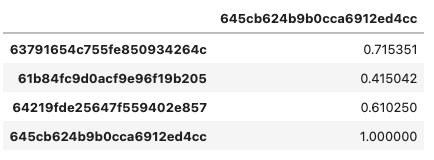
\includegraphics[width=1\textwidth, center]{dbscan_results_2_1.png}
    \caption[DBScan Ergebnisse der RevPAR-Korrelationen für das zweiten Benchmark-Hotel]{DBScan Ergebnisse der RevPAR-Korrelationen für das zweite Benchmark-Hotel}
    \label{img:dbscan_results_2_1}
\end{figure}

Die Evaluation des Hotels mit der ID \emph{645cb624b9b0cca6912ed4cc} ergab, dass die Anforderungen an einen Korrelationswert von mindestens 0,8 nicht erfüllt wurden. Somit lässt sich ableiten, dass die Ähnlichkeit der Merkmale zwischen den einzelnen Hotels nicht zwangsläufig mit der Ähnlichkeit in Bezug auf die RevPAR-Werte in Verbindung steht. 
\newline
\newline
Obwohl der DBScan-Algorithmus im Vergleich zum Basismodell verbesserte Ergebnisse lieferte, bleibt das Gesamtergebnis dennoch unbefriedigend. Besonders bedenklich ist dabei, dass die überwiegende Mehrheit der Hotels keinem Cluster zugeordnet werden konnten.


\section{Doc2Vec Modell}
\label{subsubsec:doc2vec}
In Anbetracht des unbefriedigenden Ergebnisses des DBScan-Algorithmus wird nun die Erprobung eines weiteren Modells in Betracht gezogen, um ähnliche Hotels zu identifizieren. Die nächste Alternative besteht in der Anwendung des Doc2Vec-Modells.
\newline
\newline
Doc2Vec ist ein maschinelles Lernverfahren, das dazu dient, Dokumente in einem kontinuierlichen Vektorraum abzubilden. Es wurde als Weiterentwicklung von Word2Vec konzipiert, einem etablierten Ansatz zur Repräsentation von Wörtern in einem semantischen Vektorraum. Das Hauptziel von Doc2Vec besteht darin, eine kontinuierliche Darstellung von Dokumenten zu generieren, um semantische Ähnlichkeiten zwischen diesen Dokumenten zu erfassen \cite{LeV.16.05.2014}.
\newline
\newline
Die grundlegende Idee besteht darin, jedes Hotel in einem textbasierten Dokument zu repräsentieren und dem Doc2Vec-Modell die Aufgabe zu übertragen, ähnliche Dokumente zu identifizieren. Dieser Ansatz zielt darauf ab, zu verhindern, dass Hotels ohne jegliche Zuordnung zu anderen Hotels vorliegen.
\newline
\newline
Ähnlich wie beim DBScan, wo der Vorteil darin bestand, keine Cluster angeben zu müssen, weist auch das Doc2Vec-Modell den Vorteil auf, dass keinerlei Cluster explizit angegeben werden müssen. Zudem eröffnet sich hier ein weiterer Vorteil, der beim DBScan-Algorithmus nicht gegeben war. Die beiden Informationen \emph{Art} und \emph{Region} sind beide durch Strings repräsentiert. Da Doc2Vec mit einer textbasierten Repräsentation arbeitet, bedarf es keiner Umwandlung dieser beiden Merkmale mittels \emph{One-Hot-Encoding}.

\subsection{Vorbereitung des Datensatzes} 
Auch in diesem Kontext erfordert der in Abbildung \ref{img:all_features_4} dargestellte Datensatz eine vorherige Verarbeitung, um mit dem Doc2Vec-Modell kompatibel zu sein. Die Vorbereitung besteht darin, dem Datensatz eine zusätzliche Spalte hinzuzufügen, die sämtliche Informationen des Hotels als textbasiertes Dokument repräsentiert. 
\newline
\newline
Im Folgenden wird eine Hilfsfunktion präsentiert, die dazu dient, die textbasierten Dokumente anhand der einzelnen Informationen zu erstellen.

\begin{lstlisting}[language=Python, label=lst:doc2vec_hilfs_func, caption=Hilfsfunktion zur Erzeugung von textbasierten Dokumenten]
# Copy the dataset to keep the original clean
doc2vec_df = df.copy()
    
# Get the columns of the dataset dynamic
column_names = doc2vec_df.columns
    
# Function to generate the document out of each columns
def concatenate_columns(row):
    result = "Hoteleigenschaften: "
    for column in column_names:
        result += column + "=" + str(row[column]) + " "
    return result
    
# Add the document in a new column "doc"
doc2vec_df['doc'] = doc2vec_df.apply(concatenate_columns, axis=1)
\end{lstlisting}

Durch die im Listing \ref{lst:doc2vec_hilfs_func} präsentierten Codezeilen, wurde dem Datensatz eine neue Spalte namens \emph{doc} hinzugefügt, die später als Eingabe für das Modell dienen soll. Zur Veranschaulichung dieser neu erstellten \emph{doc}-Spalte soll das erste Dokument als Beispiel dienen:

\begin{figure}[h]
    \centering
    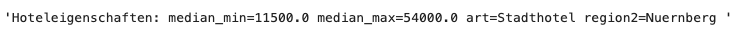
\includegraphics[width=1\textwidth, center]{ex_doc.png}
    \caption[Exemplarisches Dokument innerhalb des Datensatzes]{Exemplarisches Dokument innerhalb des Datensatzes}
    \label{img:ex_doc}
\end{figure}

Mithilfe dieser neuen Repräsentation kann nun im nächsten Schritt das Modell trainiert werden.

\subsection{Modellbildung}

Nach der erfolgten Datenvorbereitung und der Erstellung der textbasierten Dokumente für jedes Hotel kann das Modell nun trainiert werden. Hierzu werden die Hotel-IDs zunächst als Index festgelegt. Anschließend wird der Datensatz in sogenannte \emph{TaggedDocument} Objekte umgewandelt. Diese \emph{TaggedDocument} Objekte erfassen die einzelnen Wörter innerhalb eines Dokuments sowie ein sogenanntes \emph{Tag}, welches zur Identifikation des jeweiligen Dokuments dient. In diesem Kontext repräsentiert das \emph{Tag} die Hotel-ID. Der letzte Schritt besteht darin, die \emph{TaggedDocument} Objekte unter Verwendung einiger Hyperparameter dem Modell zuzuführen und das Training zu starten. Sobald das Modell trainiert ist, können ähnliche Dokumente zu einem ausgewählten Dokument, das durch die Hotel-ID identifiziert wird, gefunden werden.
\newline
\newline
Dieses Verhalten wird im nachfolgenden Listing dargestellt:
\begin{lstlisting}[language=Python, label=lst:doc2vec_exe, caption=Ausführung des Doc2Vec Modell]
# Generate the TaggetDocuments with Hotel-ID as Tag
documents = [TaggedDocument(words=doc.split(), tags=[str(i)]) for i, doc in doc2vec_df["doc"].iteritems()]
    
# Train the Model
model = Doc2Vec(documents, vector_size=10, window=3, min_count=1, workers=4, epochs=1000, alpha=0.01)
    
# Get similar documents als tupel (ID, Doc)
similar_documents = model.dv.most_similar(str(benchmark_hotel_id), topn=4)
    
pred_hotel_ids = [tupel[0] for tupel in similar_documents]
\end{lstlisting}

Nun stehen in der Variable \emph{pred\_hotel\_ids} die Hotel-IDs, die anhand von dem Doc2Vec Modell als am ähnlichsten empfunden wurden. Diese können wie auch schon beim DBScan Algorithmus anhand ihrer Merkmale betrachtet werden.

\begin{figure}[h]
    \centering
    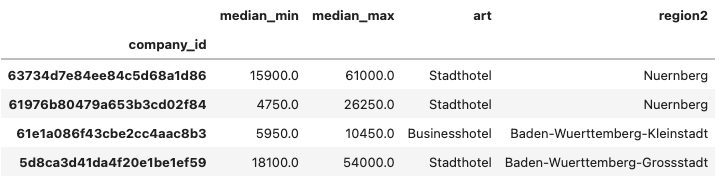
\includegraphics[width=1\textwidth, center]{doc2vec_hotels_1.png}
    \caption[Gefundene Hotels für das erste Benchmark-Hotel mit dem Doc2Vec Modell]{Gefundene Hotels für das erste Benchmark-Hotel mit dem Doc2Vec Modell}
    \label{img:doc2vec_hotels_1}
\end{figure}

Es zeigt sich, dass das Doc2Vec Modell ganz andere Hotels als ähnlich identifiziert hat. Im Gegensatz zum DBScan-Algorithmus scheinen die Merkmale der gefundenen Hotels lediglich Überlappungen aufzuweisen, anstatt sich zu teilen. Wie bereits in den vorhergehenden Abschnitten ersichtlich wurde, müssen sich die Merkmale nicht zwangsläufig überschneiden.

\subsection{Evaluation}
Ungeachtet der jeweiligen Merkmale der einzelnen Hotels besteht die Möglichkeit, dass diese dennoch Ähnlichkeiten in dem RevPAR-Verlauf aufweisen. Diese Annahme soll im Folgenden überprüft werden.

\begin{figure}[h]
    \centering
    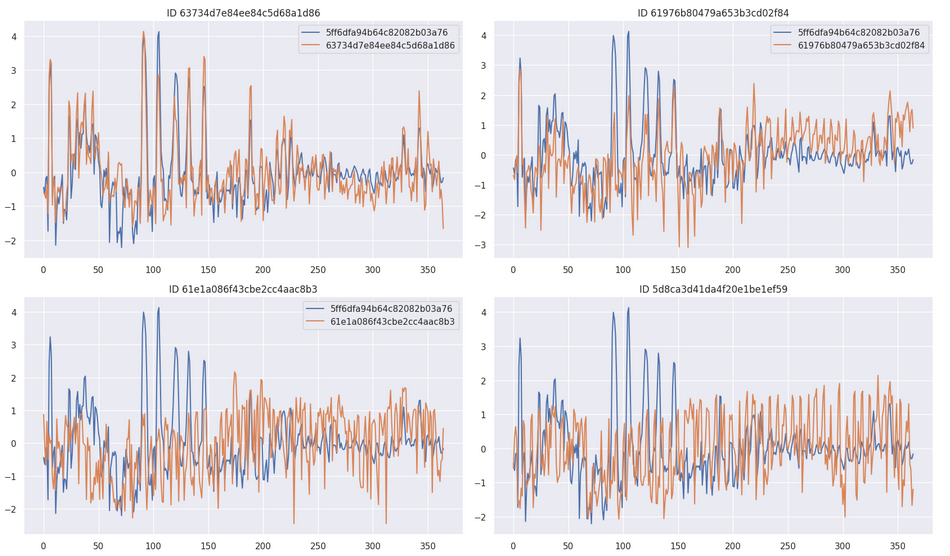
\includegraphics[width=1\textwidth, center]{doc2vec_results_1.png}
    \caption[Doc2Vec Ergebnisse der RevPAR-Verläufe für das erste Benchmark-Hotel]{Doc2Vec Ergebnisse der RevPAR-Verläufe für das erste Benchmark-Hotel}
    \label{img:doc2vec_results_1}
\end{figure}

\begin{figure}[h]
    \centering
    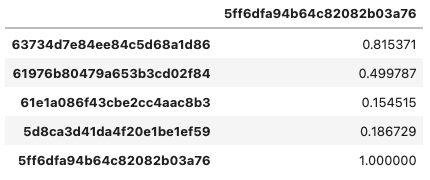
\includegraphics[width=0.5\textwidth, center]{doc2vec_results_1_1.png}
    \caption[Doc2Vec Ergebnisse der RevPAR-Korrelationen für das erste Benchmark-Hotel]{Doc2Vec Ergebnisse der RevPAR-Korrelationen für das erste Benchmark-Hotel}
    \label{img:doc2vec_results_1_1}
\end{figure}

Es offenbart sich, dass das Doc2Vec-Modell erheblich schlechter abschneidet als der DBScan-Algorithmus. Diese Feststellung wird bereits anhand des ersten Benchmark-Hotels ersichtlich, und es wird daher auf die detaillierte Evaluation dieses Benchmark-Hotels verzichtet.
\subsubsection{Unbewachtes Lernen Fazit}
\label{subsubsec:un_fazit}
Sowohl der Einsatz des DBScan-Algorithmus als auch der Ansatz des Doc2Vec-Modells haben sich als unzureichend erwiesen. Trotz der Identifikation von Hotels in beiden Ansätzen lässt sich im Vorfeld nicht sicherstellen, ob diese tatsächlich als ähnlich zueinander betrachtet werden können. Aufgrund dieser Erkenntnisse wurde die Entscheidung getroffen, beide Ansätze zu verwerfen und eine neue Methodik zur Identifizierung ähnlicher Hotels zu entwickeln.